\renewcommand{\captiontitle}{\omeganet{} 网络结构概览}
\begin{figure*}
\begin{center}

\begin{tikzpicture}
\newcommand{\tw}{\textwidth}

\node [anchor=south west] (image) at (0,0) {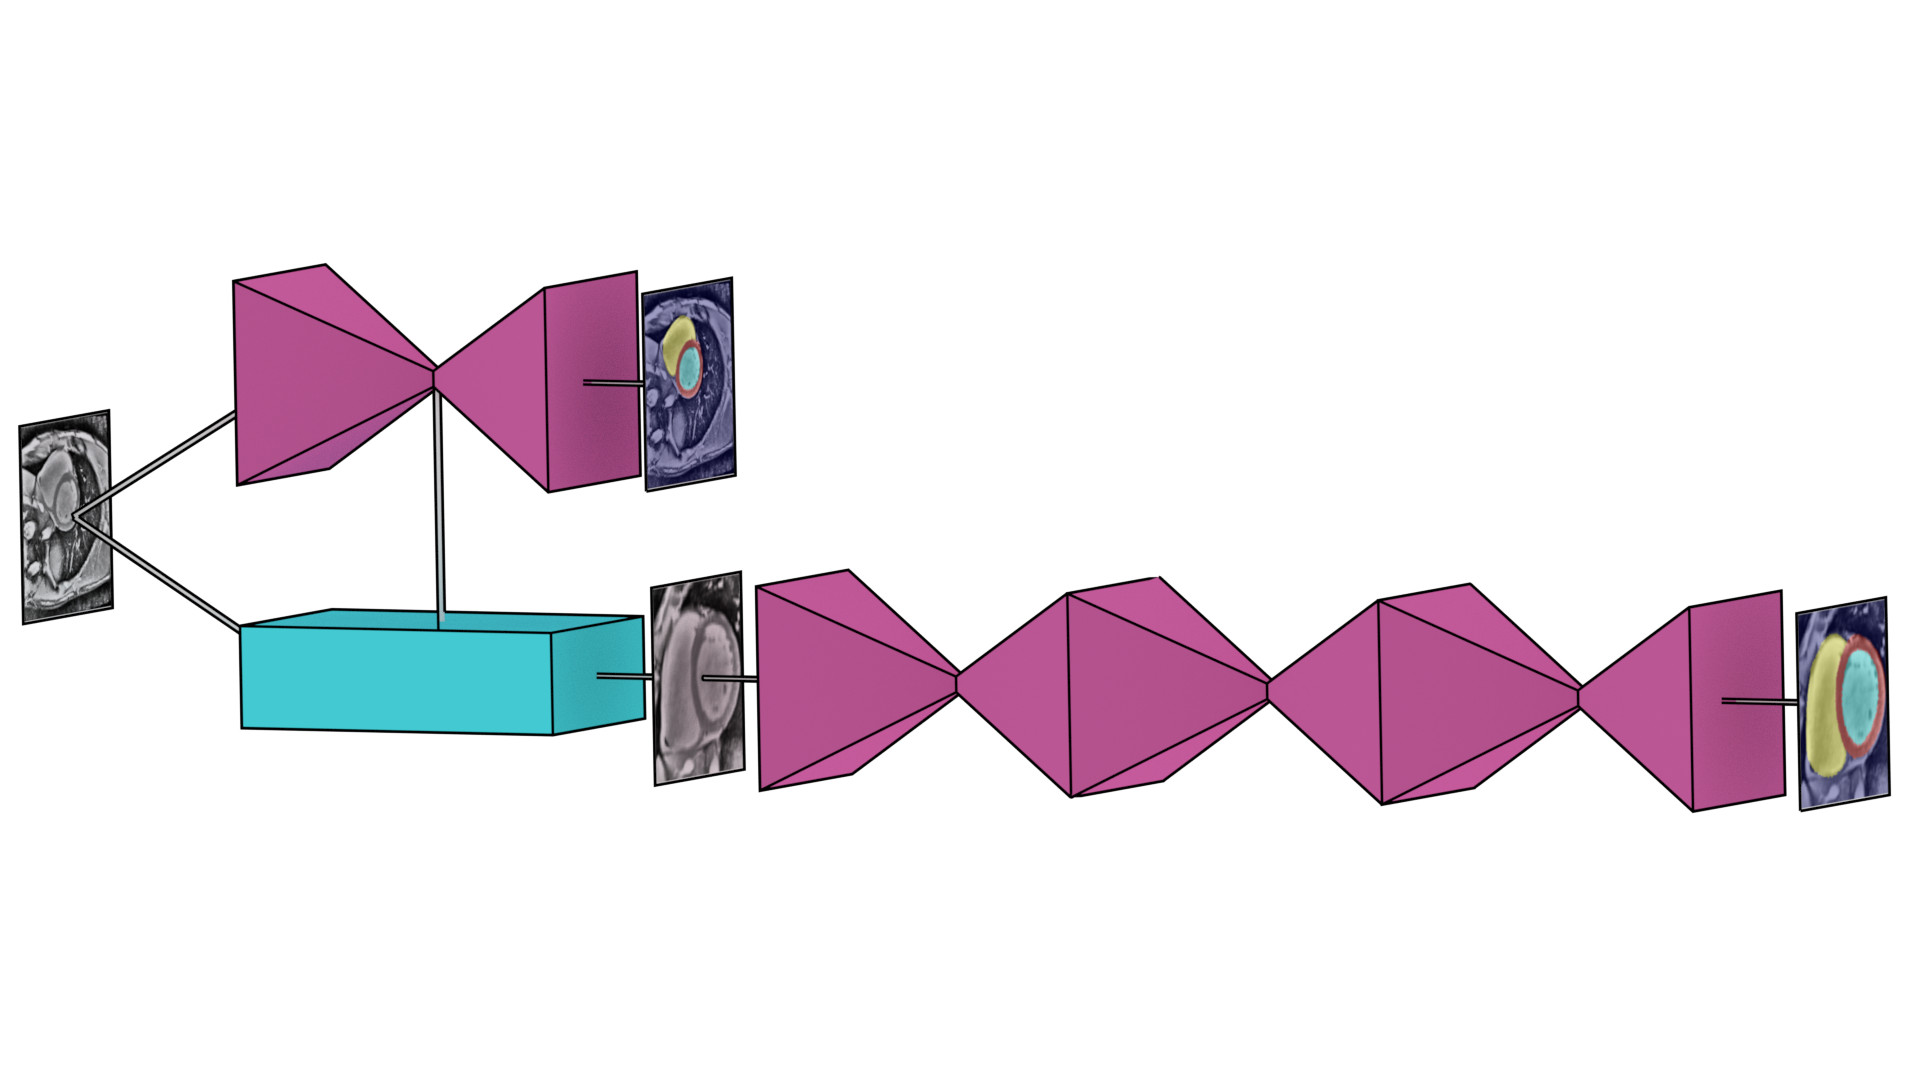
\includegraphics[clip, trim=0 260 0 260, width=1.0\textwidth]{./data/ohm-net-architecture.png}};

\node [anchor=south west] (a) at (0.025\tw,0.22\tw) {\large $\image$};
\node [anchor=south west] (b) at (0.35\tw,0.13\tw) {\large $\image^\prime$};
\node [anchor=south west] (c) at (0.35\tw,0.29\tw) {\large $S$};
\node [anchor=south west] (d) at (0.95\tw,0.13\tw) {\large $S^\prime$};
\node [anchor=south west] (e) at (0.17\tw,0.06\tw) {\large $\trans(\image, \tmat)$};

\draw [decorate,decoration={brace,amplitude=10pt},xshift=0pt,yshift=0pt](0.1275\tw,0.3\tw) -- (0.34\tw,0.3\tw) node [black,midway,xshift=0.0cm,yshift=+0.7cm] {(a) 粗分割模块};
\draw [decorate,decoration={brace,amplitude=10pt},xshift=0pt,yshift=0pt](0.3425\tw,0.045\tw) -- (0.1325\tw,0.045\tw) node [black,midway,xshift=0.0cm,yshift=-0.7cm] {(b) 变换模块};
\draw [decorate,decoration={brace,amplitude=10pt},xshift=0pt,yshift=0pt](0.4\tw,0.15\tw) -- (0.935\tw,0.15\tw) node [black,midway,xshift=0.0cm,yshift=+0.7cm] {(c) 细分割模块};
\end{tikzpicture}

\caption[\captiontitle]{\captiontitle{}.  (a) 将原始的 \SSFP{} 图像送入 \UNet{} 模块,得到一个粗分割输出 $S$.(b) 从该层 \UNet{} 中间(下采样)层输出的特征被用来给变换模块预测一个刚体仿射变换的参数 $\tmat$,该变换这可将输入图像变换到一个典型方向 $\image^\prime = \trans(\image, \tmat)$.(c) 这个变换后的图像就送入一个对堆叠的沙漏形网络对变换到典型方向的 $S^\prime$ 进行最后的细分割.需要说明的是,这里的所有模块都是从头开始端到端的训练的.}
\label{fig:omega-net-architecture}
\end{center}
\end{figure*}


二维静态图像序列(SSFP, steady state free precession)的左心和四腔心分割是进行容量估计(如射血分数,每搏量和心输出量);形态学特征(如心肌质地,壁厚等)和应力分析\citep{Peng2016}前的必要步骤.
然而,心脏的全自动分割依然是一个棘手的问题,主要是因为:

\begin{itemize}
\item 心脏大小、方向以及形态学上的生物差异.
\item 不同扫描仪器、流程和临床切面的对比度和外观差异.
\item 心内膜小梁和乳头肌的影响.
\item 心室心房之间以及心腔和血管之间的模糊边界
\end{itemize}

解决上述问题常用的有三种方法.
第一,对问题的范围进行限定,例如只对 SA 切面的左心肌和血池进行分割.
第二,增加用户交互,提供有效的初始化,额外的解剖标记或者错误修正.
第三,将心脏结构的先验知识融合到模型中.
显然,这些方法都不够理想:第一种方法限制了算法能够学习到的信息;第二种方法增加了医生的劳动;而第三种方法需要更加小心的设计算法. 

近来,深度神经网络\hl{CNNs}在自然图像分类\hl{\citep{Krizhevsky2012,Simonyan2015}}和分割\citep{Long2015,Noh2015,Yu2016}以及生物医学图像分析\citep{Ronneberger2015,Xie2015}取得瞩目的成就.
已有研究将 CNN 分割应用到短轴切面 CMR 图像的左室血池(\citep{Tan2016,Poudel2016a,Tan2017}),右室血池(\citep{Luo2016}),以及同时对前述两者分割(\citep{Tran2016,Lieman-Sifry2017,Vigneault2017}).
这些方法要么定位和分割是分别进行\citep{Tan2016, Poudel2016a, Tan2017, Luo2016},要么是预先对图像进行裁剪,使得心脏就在图像中央,并占图像的主要部分,从而避开了定位任务\hl{\citep{Tran2016, Lieman-Sifry2017, Vigneault2017}}.他们都没有做端到端的定位和分割,也没有先变换到一个典型方向再做分割.

\renewcommand{\captiontitle}{典型方向下的临床切面}
\begin{figure*}
\begin{center}

\setlength{\tabcolsep}{1pt}

\begin{tabular}{ccccc}

\toprule
\SA{}(底层切片) & \SA{}(中间切片) & \SA{}(顶层切片) & \HLA{} & \VLA{} \\
\midrule

\multicolumn{5}{c}{未对齐方向的原始图像: $\image$} \\

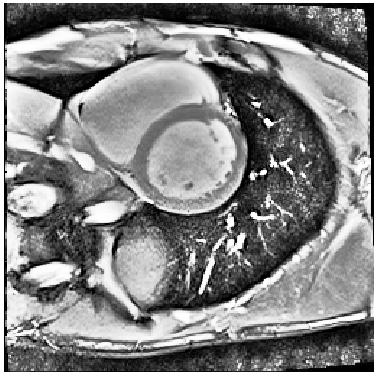
\includegraphics[width=0.19\textwidth]{./data/ohm/control/HCMNet_1100594/00_SAX/35_/im.png} &
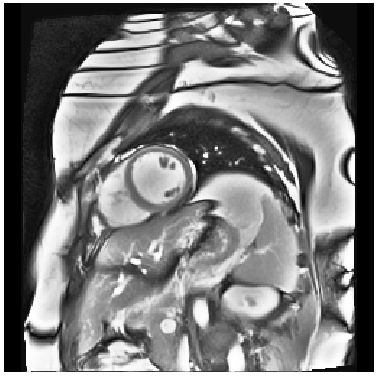
\includegraphics[width=0.19\textwidth]{./data/ohm/control/HCMNet_1100823/00_SAX/33_/im.png} &
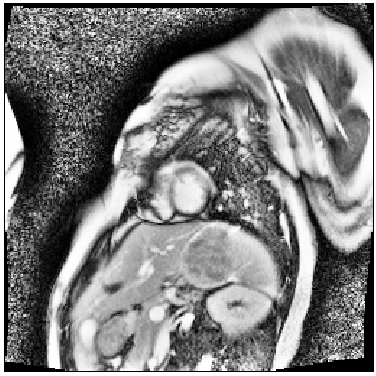
\includegraphics[width=0.19\textwidth]{./data/ohm/control/HCMNet_2600035/00_SAX/024_SA_CINE/im.png} &
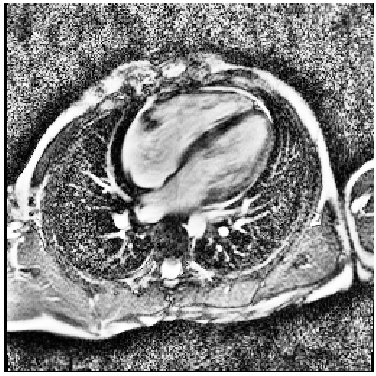
\includegraphics[width=0.19\textwidth]{./data/ohm/control/HCMNet_1700012/01_HLA/00/im.png} &
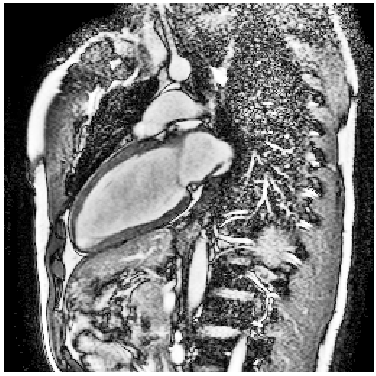
\includegraphics[width=0.19\textwidth]{./data/ohm/control/HCMNet_2100096/02_VLA/00/im.png} \\

\multicolumn{5}{c}{结构定位} \\

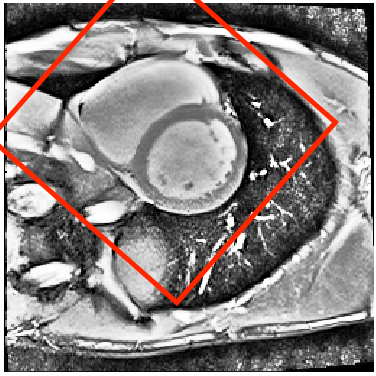
\includegraphics[width=0.19\textwidth]{./data/ohm/control/HCMNet_1100594/00_SAX/35_/im_det.png} &
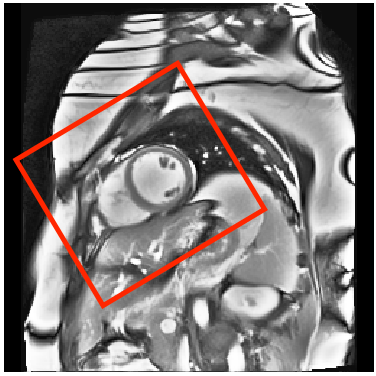
\includegraphics[width=0.19\textwidth]{./data/ohm/control/HCMNet_1100823/00_SAX/33_/im_det.png} &
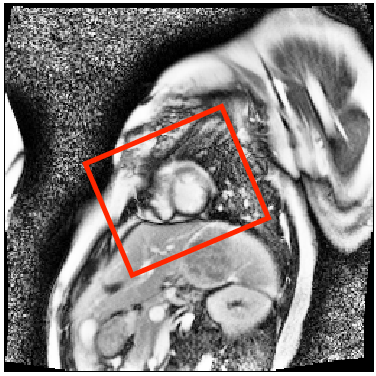
\includegraphics[width=0.19\textwidth]{./data/ohm/control/HCMNet_2600035/00_SAX/024_SA_CINE/im_det.png} &
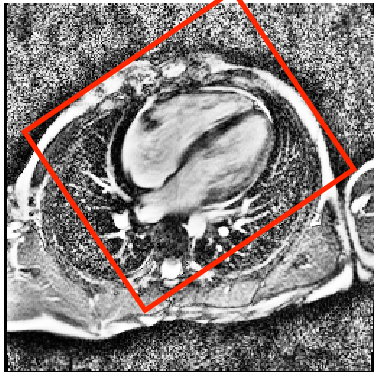
\includegraphics[width=0.19\textwidth]{./data/ohm/control/HCMNet_1700012/01_HLA/00/im_det.png} &
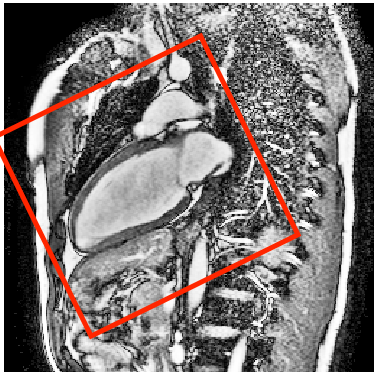
\includegraphics[width=0.19\textwidth]{./data/ohm/control/HCMNet_2100096/02_VLA/00/im_det.png} \\

\multicolumn{5}{c}{变换到典型方向的图像:$\image^\prime = \trans(\image,M)$} \\

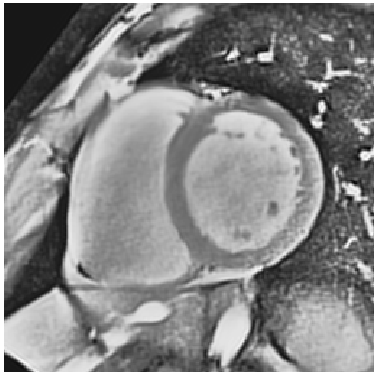
\includegraphics[width=0.19\textwidth]{./data/ohm/control/HCMNet_1100594/00_SAX/35_/im_t.png} &
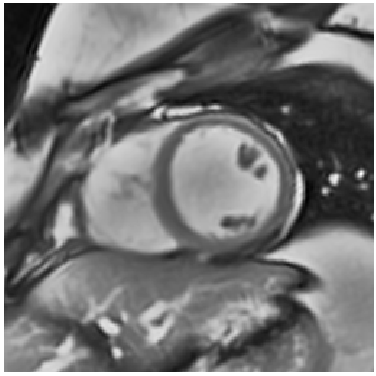
\includegraphics[width=0.19\textwidth]{./data/ohm/control/HCMNet_1100823/00_SAX/33_/im_t.png} &
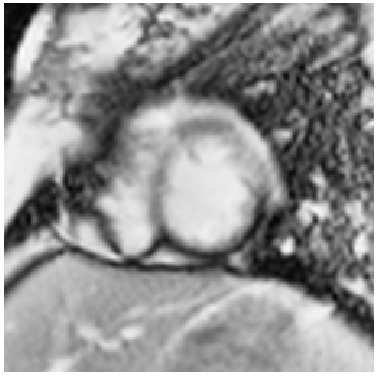
\includegraphics[width=0.19\textwidth]{./data/ohm/control/HCMNet_2600035/00_SAX/024_SA_CINE/im_t.png} &
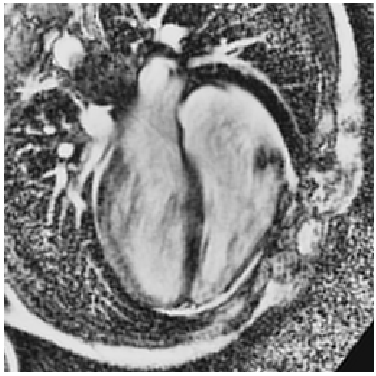
\includegraphics[width=0.19\textwidth]{./data/ohm/control/HCMNet_1700012/01_HLA/00/im_t.png} &
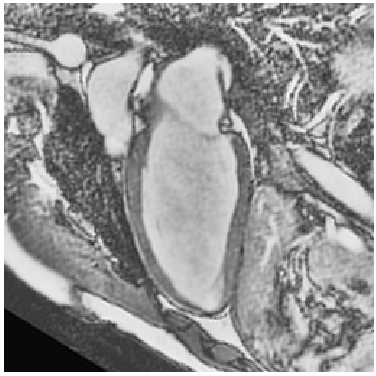
\includegraphics[width=0.19\textwidth]{./data/ohm/control/HCMNet_2100096/02_VLA/00/im_t.png} \\
\bottomrule

\end{tabular}

\caption[\captiontitle]{\captiontitle{}.
图中上面一行为短轴面(\SA{})、四腔切面(\HLA{})和两腔(\VLA{})的图像,下面一行为对应的经过一个刚体、仿射变换后变换到一个典型方向的图像.
按照临床习惯,心脏已经经过了旋转,使得 \SA{} 面的右室在放射学上的图像右侧,而左室在 \HLA{} 和 \VLA{} 面的方向是沿着长轴方向的.
心脏区域也已经移中并缩放,占到图像大小的 $90\%$.
请注意未经过方向对齐的图像中心脏的大小、方向和外观的异质,这大大增加了分割的难度.
}
\label{fig:canonical-orientation}
\end{center}
\end{figure*}


\hl{
在深度学习领域,CNN 网络的不变性仅仅是来自平均化池化和最大化池化的组合.
然而,卷积或者相关操作有几个缺陷:它既不是旋转不变或等变的,也不是尺度不变的,因此需要需要大量的数据来表示这些可能的变化 \citep{Sifre2013, Dieleman2015}.
}
在本文中,我们提出 \omeganet{}(Omega-Net),一个全新的 CNN 网络架构,来解决这三个问题(图 \ref{fig:omega-net-architecture}).

简单起见,尽管更加复杂的网络,例如 ResNet \citep{He2016} 也可以使用,我们还是使用 \UNet{} 作为粗分割和细分割的组成模块 \citep{Ronneberger2015}.
受空间变换网络 \citep{Jaderberg2015} 的启发,我们设计了一个完全不同的网络来实现定位和变换到一个典型方向的功能.

变换后的图像被送入一个由沙漏形网络堆叠而成的细分割网络 \citep{Newell2016}.
\hl{
在这样一个堆叠的沙漏形网络中,多个 \UNet{} 模块完成分割,并将输出传到下一个 \UNet{} 中.
这样的结构已经被证明可以逐渐降低误差,提升准确率 \citep{Newell2016}.
}

我们展示了 \omeganet{} 可以进行全自动的分割出三个标准切面(SA,短轴面;4C,四腔心面;2C,两腔心面)中的五个前景类别(左室心肌,左右心房和左右心室),参见图 \ref{fig:canonical-orientation}.
而且,我们的网络在多中心点的患者上测试,这些患者患有肥厚性心肌病(\HCM{}).这大大增加了问题的难度与复杂性,因为左室的巨大差异.
网络性能,以 \IoU{} 计算,比起没有使用定位和方向变换的 \UNet{} 分割结果有明显的提升($0.858$ vs $0.834$).
\hl{
此外,我们在 2017 MICCAI 自动心脏病诊断挑战公开数据集上(\miccaidata{}) dataset,\footnote{\url{https://www.creatis.insa-lyon.fr/Challenge/acdc/}}从头开始训练,并取得了比现有结果\citep{Isensee2018}更好的成绩,仅有左室心肌的分割略差.
}
